\documentclass[conference,a4paper]{IEEEtran}
\usepackage{cite}
\usepackage{amsmath}
\usepackage{graphicx}
\usepackage{textcomp}
\usepackage{booktabs}
\usepackage{array}
\usepackage{url}

\begin{document}

\title{C3: Browser-Execution-Aware Detection of Command-and-Control Beacons Under Leakage-Free Evaluation}

\author{
\IEEEauthorblockN{L. K. Wadduwage, Hansika Mahaadikara, Amila Senarathne}
\IEEEauthorblockA{Department of Computer Systems Engineering\\
Sri Lanka Institute of Information Technology, Malabe, Sri Lanka\\
it22208408@my.sliit.lk, hansika.m@sliit.lk, amila.s@sliit.lk}
}

\maketitle

\begin{abstract}
A browser extension or a compromised web page that beacons to a command-and-control (C2) server produces periodic HTTPS requests that are indistinguishable from ordinary browsing at the network-flow level. We present C3, a detector that observes outbound requests inside a managed browser through the DevTools Protocol, labels each request with browser-execution context that no network capture can supply -- user activity, tab visibility, and request initiator -- and fuses a calibrated gradient-boosted classifier with nine deterministic rules. Our principal contribution is methodological. Evaluating by unseen malware family and by unseen C2 infrastructure, rather than by a random split, exposed two defects in the training corpus: one family's positive windows were 95\% drawn from a single communicating pair, and that same capture was a non-periodic dead-server retry storm labelled as a beacon. We diagnose both, define a scope criterion that is independent of the timing features used for detection, and correct a threshold-placement bug introduced by calibration. On the corrected corpus, under one reliability rule applied uniformly to both protocols, the deployed model reaches 92.3\% accuracy and 0.978 ROC-AUC on unseen C2 infrastructure and 83.8\% accuracy and 0.927 ROC-AUC on an unseen malware family, class-balanced and leakage-free.
\end{abstract}

\begin{IEEEkeywords}
command-and-control detection, browser security, dataset leakage, probability calibration, behavioral anomaly detection
\end{IEEEkeywords}

\section{Introduction}

Command-and-control beaconing is the step that turns a compromise into an operation: the implant contacts its server on a schedule, receives instructions, and returns results. Detection has traditionally been treated as a network problem and solved by looking for regularity -- consistent inter-arrival times, consistent payload sizes, and a destination contacted at a cadence no human would produce \cite{garcia2014ctu13, gu2008botminer, bilge2012disclosure}. Beaconing is a named and persistent adversary technique in attack frameworks \cite{mitre2018attack}, and malicious browser extensions remain an active and growing threat class \cite{singh2025malicious}.

When beaconing moves inside the browser -- through a malicious extension, or through script injected into a compromised page -- the network view degrades. The beacon's requests share the host's own TLS session with genuine browsing to the same destination, so a beacon to a chat platform or a document service is indistinguishable at the flow level from a user with that service open. Encryption removes the payload, and flow-level defences must fall back on side-channel features to compensate \cite{anderson2016identifying}. What the network cannot see, the browser can: whether the user was interacting with the machine when a request fired, whether the tab was in the foreground, and whether an extension rather than a page initiated the request.

The primary contribution of this paper, however, is not the architecture but what happened when we evaluated it rigorously. A classifier trained on a real, published botnet capture produced strong held-out numbers under a random train/test split. Evaluating the same model with the malware family or the specific attacker infrastructure held out entirely -- the only protocol that reflects what a deployed detector actually faces -- reduced those numbers sharply and forced us to look for the cause. We found two distinct defects in the training corpus rather than a modelling failure, and a further bug specific to the probability calibration added to correct one of them. Concretely, we contribute:

\begin{itemize}
\item A non-invasive, browser-execution-aware collector built on the Chrome DevTools Protocol, producing a 29-feature per-host vector: 18 scale-free features that the classifier reads, and 11 context or absolute-scale signals used only by a deterministic heuristic layer, fused with fixed, measured weights (Section III).
\item Diagnosis and correction of \emph{pseudo-replication} -- one malware family's positive windows were 95\% drawn from a single communicating pair, that is, one session rather than the independent evidence a window count implies -- and of an \emph{out-of-scope concept} inside the positive class, a non-periodic dead-C2 retry storm, removed by a scope criterion defined independently of the timing features used for detection (Section IV).
\item A threshold-placement bug specific to isotonic calibration, in which a naive quantile rule is invalidated by the tied outputs that calibration produces, isolated in an ablation on identical data (Section V).
\item Leakage-free evaluation by unseen family and by unseen C2 source, with a single reliability rule applied uniformly to both protocols, reported alongside a five-classifier comparison that shows \emph{why} the deployed classifier was selected rather than merely that it was: an alternative wins the optimistic split and then generalises to zero (Section VI).
\item A measured structural result: with fixed fusion weights, a confirmed detection is unreachable from the learned signal alone at any tested weight once browser context is unavailable. This is a property of the fusion architecture, not an artefact of training (Section VI-D).
\end{itemize}

\section{Related Work}

\textbf{Flow-based detection.} Regularity statistics over inter-arrival times, payload-size consistency, and destination entropy underpin both academic and production beacon detectors. The CTU-13 capture set \cite{garcia2014ctu13} remains a standard labelled corpus for this line of work; clustering communication and activity patterns independently of protocol was established by Gu \emph{et al.} \cite{gu2008botminer}, and Bilge \emph{et al.} showed that C2 servers can be identified from NetFlow records at scale \cite{bilge2012disclosure}. More recent work applies unsupervised decoding directly to beaconing periodicity for threat hunting \cite{mahboubi2025lurking}. None of this literature has browser execution context available to it, by construction: it operates on network captures.

\textbf{Browser-mediated threats.} Malicious browser extensions are an active and growing category, and recent large-scale studies characterise their behaviour and prevalence \cite{singh2025malicious}. Attributing traffic to a specific extension, tab, or script -- as opposed to the page's own first-party traffic -- is not a property that flow-level tooling can recover.

\textbf{Learning under scarce, skewed positives.} Isolation Forest \cite{liu2008isolationforest} targets precisely the setting in which labelled anomalies are scarce relative to abundant normal traffic. Gradient-boosted trees such as XGBoost \cite{chen2016xgboost} are the supervised alternative once sufficient labelled positives exist, and they are known to require explicit correction of their predicted probabilities: margin-based ensembles systematically push scores away from 0 and 1, a distortion that Niculescu-Mizil and Caruana characterise and correct with isotonic regression \cite{niculescumizil2005predicting}. That result directly motivates the calibration step in Section V.

\textbf{Evaluation bias.} A substantial security-ML literature warns that random or otherwise leakage-permissive splits over a corpus assembled from few sources overstate held-out performance. Sommer and Paxson argued early that the closed-world assumptions of standard machine-learning evaluation transfer poorly to network intrusion detection \cite{sommer2010outside}. Pendlebury \emph{et al.} formalise the problem for malware classification across space and time and argue for splits that respect the real structure of the corpus \cite{pendlebury2019tesseract}, and Arp \emph{et al.} catalogue the recurring pitfalls -- sampling bias, spurious correlations, and inappropriate performance measures among them -- across three decades of security-ML papers \cite{arp2022dos}. Our leave-one-family-out and leave-one-C2-source-out protocols apply that principle to a beacon corpus built from grouped, windowed captures. The pseudo-replication defect reported in Section IV is a concrete instance of the sampling bias these authors describe, found in our own data.

We are not aware of prior work that evaluates a browser-execution-aware C2 detector under a grouped, leakage-controlled protocol while separately auditing the training corpus itself for pseudo-replication and for label-concept scope. That is the gap this paper's evaluation methodology addresses.

\section{System Design}

\begin{figure*}[t]
\centering
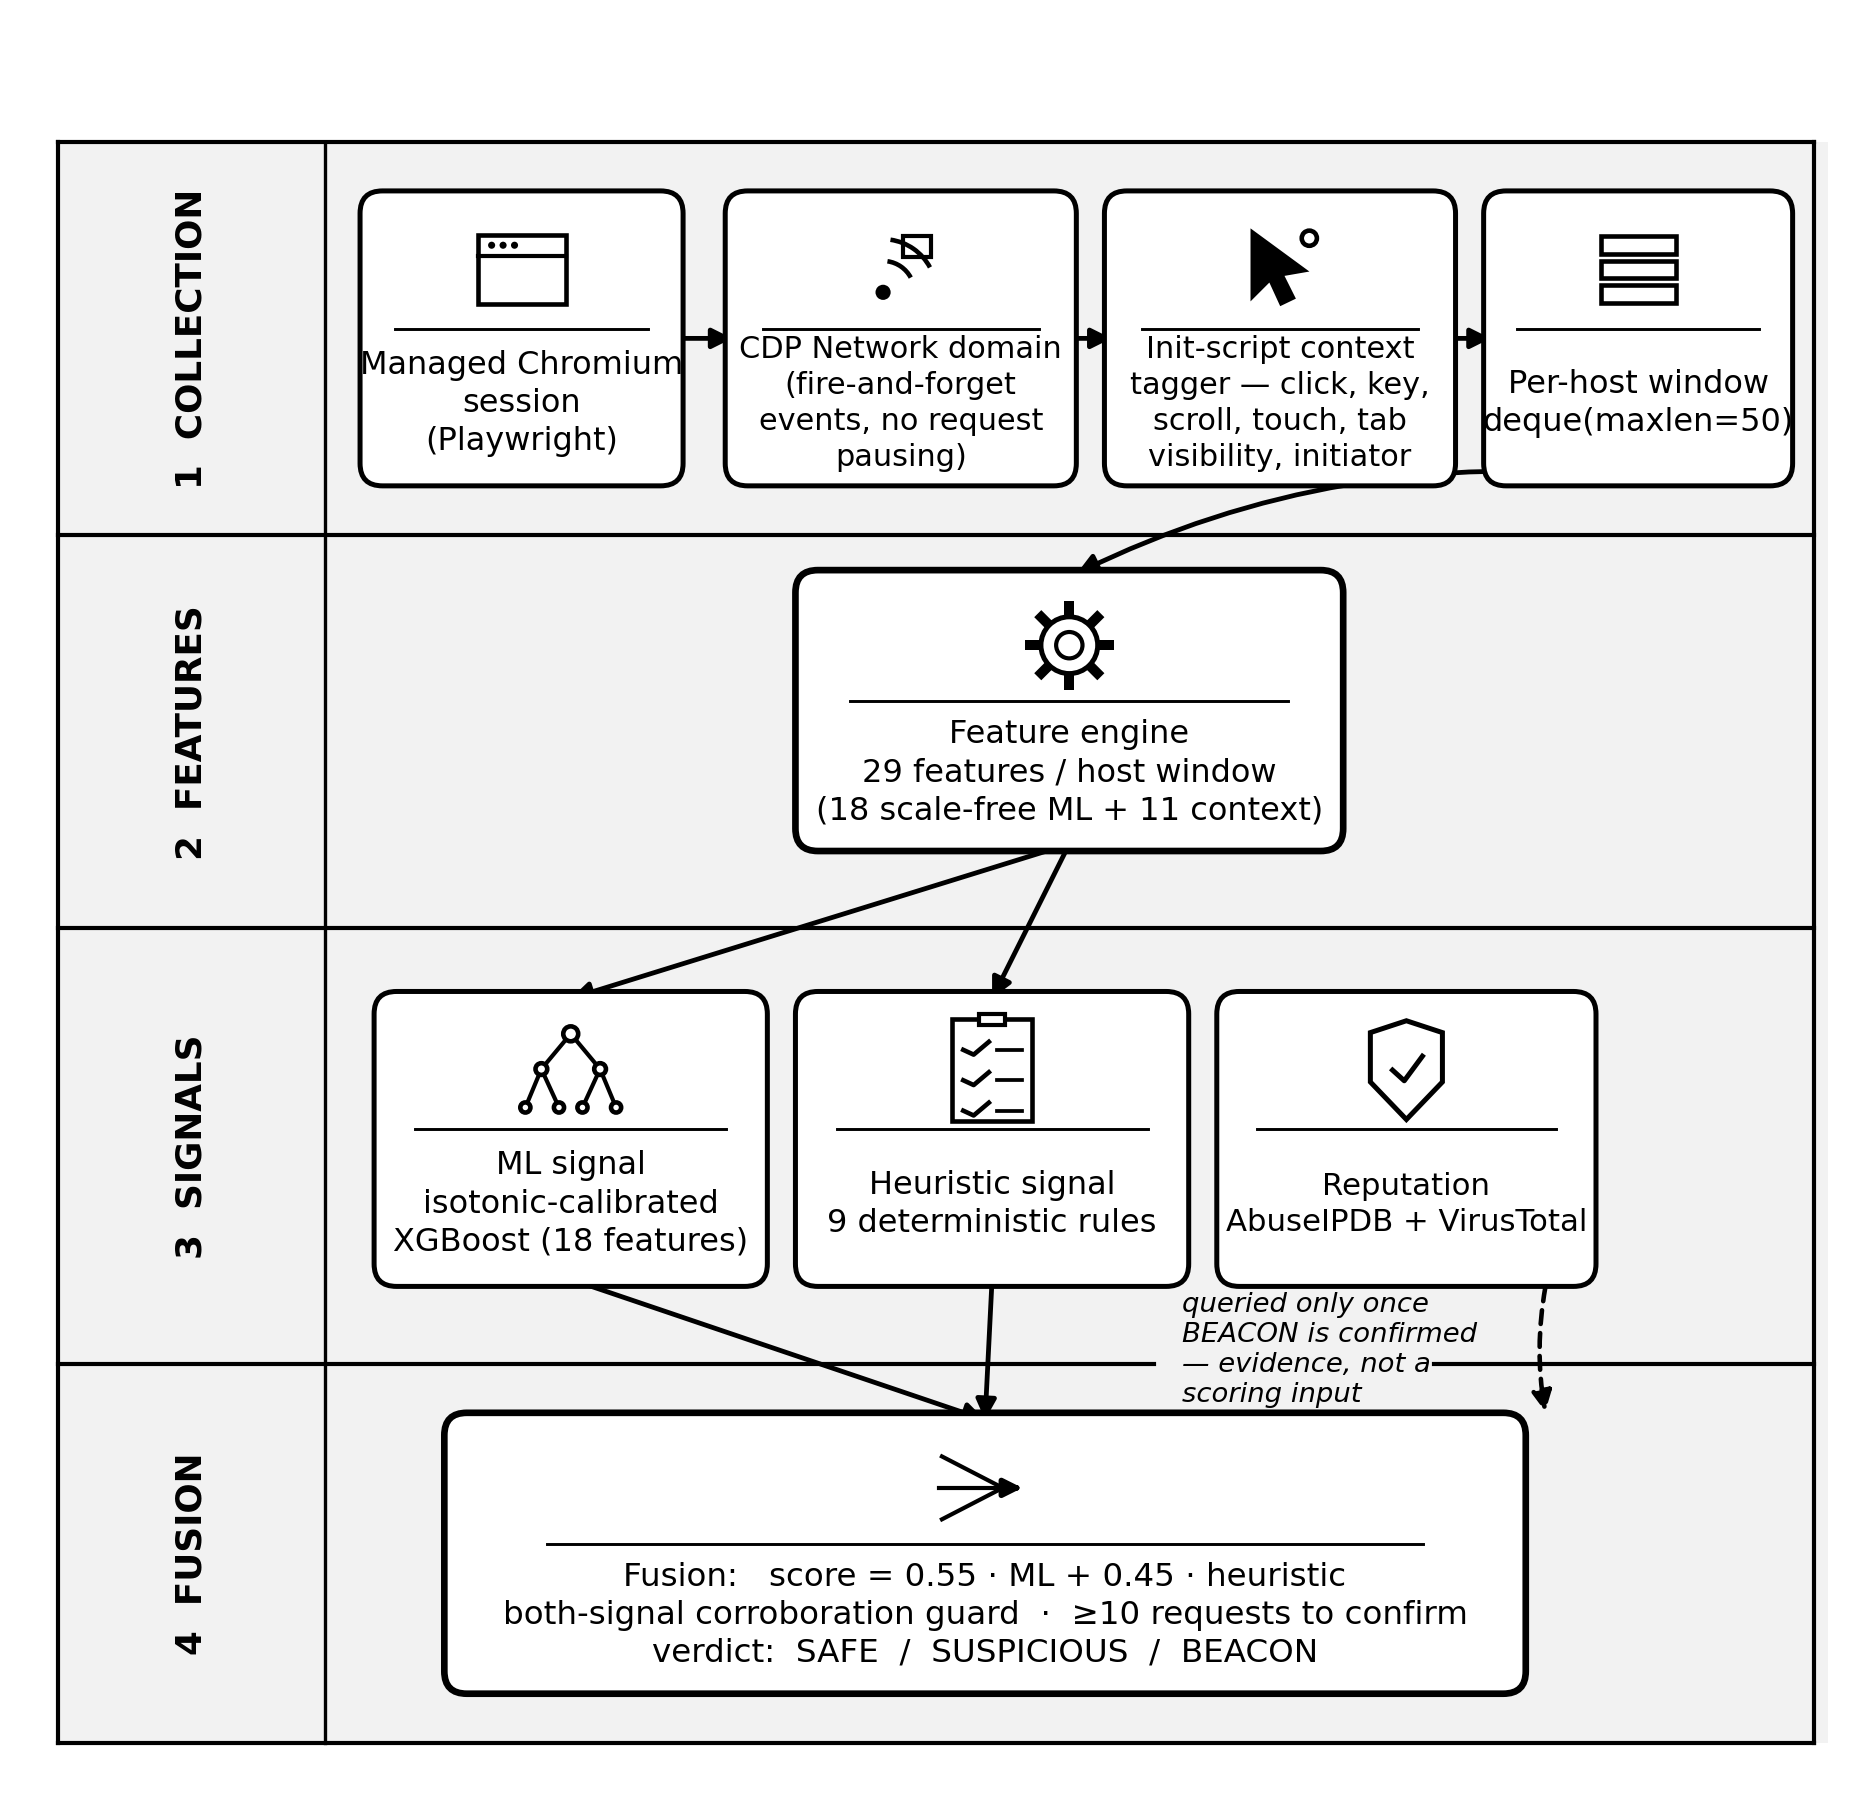
\includegraphics[width=0.86\textwidth]{figures/fig1_architecture.png}
\caption{The C3 detection pipeline. Analysis runs every 10 seconds for each monitored destination host. Reputation is consulted only after a BEACON verdict and is never an input to the score.}
\label{fig:arch}
\end{figure*}

\subsection{Non-invasive collection}
Requests are captured through the Network domain of the DevTools Protocol rather than through request interception (Fig.~\ref{fig:arch}). The distinction is a performance decision: protocol events are fire-and-forget, so the browser never waits on the analysis process, whereas a global route handler pauses every outgoing request until the handler responds \cite{chromedevtools, playwright}, which is a real cost on any page that issues many concurrent requests. User interaction (click, keydown, scroll, and touchstart) and tab visibility are recorded by an init script. Pointer movement is deliberately excluded, because it fires from passive cursor presence and inflates measured activity for exactly the two features that matter most for this task. Requests from service workers and other non-page contexts are attributed to the background with the user marked inactive, which computes context correctly without requiring a page to compare against.

\subsection{Feature vector}
Every 10 seconds, the rolling window of up to 50 requests for each destination host -- a fixed-size deque, from which the oldest requests are dropped -- is reduced to 29 features. Eighteen of them are scale-free (ratios, shares, and normalised entropies) and are the only features the classifier reads (Table \ref{tab:features}); using absolute byte counts or absolute intervals was found to teach the model the specific scale of a 2011 capture rather than the property of beaconing, as discussed in Section IV. The most important trained feature, at 31.8\% of total gain, is not a timing statistic at all: it is the share of requests that carry no \texttt{Referer} header, because a timer-fired request is not the result of a click and carries none. The remaining 11 features (mean and MAD inter-arrival time, request-burst count, requests per hour, same-site ratio, script-initiator ratio, and four browser-context fields) drive the deterministic heuristic layer directly. They are absolute-scale or context features that no offline network corpus can label.

\begin{table}[t]
\caption{The 18 scale-free ML features, by group, with trained importance}
\label{tab:features}
\centering
\small
\setlength{\tabcolsep}{3pt}
\begin{tabular}{p{0.20\columnwidth}p{0.58\columnwidth}c}
\toprule
\textbf{Group} & \textbf{Features} & \textbf{Imp.} \\
\midrule
Timing shape (8) & inter-arrival CV, Bowley skewness, normalized MAD, burstiness, lag-1 autocorrelation, spread ratio, clock-boundary share, normalized entropy & 29.8\% \\
Payload size (4) & mean, coefficient of variation, size-repeat ratio, upload/download ratio & 19.6\% \\
URL / method (5) & path entropy, unique-path ratio, POST ratio, normalized URI length, URI character entropy & 18.8\% \\
Request behaviour (1) & Referer-absent ratio & \textbf{31.8\%} \\
\bottomrule
\end{tabular}
\end{table}

\subsection{Heuristic layer and fusion}
Nine deterministic rules score, in turn: regular timing combined with a small payload; foreground requests firing during long user idle periods; background-tab traffic; extension-origin foreground beacon shape; low path entropy combined with regular timing and inactivity; script-initiated regularity; a high POST ratio with regular timing; a sustained high request rate while the user is inactive; and, applied last and only multiplicatively, a same-site dampener that reduces -- and never raises -- suspicion for traffic to the active page's own site, so that the legitimate background synchronisation of a single-page application is not mistaken for a beacon.

The fused score is a fixed weighted sum, \(\mathrm{score} = 0.55 \cdot \mathrm{ML} + 0.45 \cdot \mathrm{heuristic}\), mapped to SAFE ($<0.30$), SUSPICIOUS ($<0.52$), or BEACON ($\geq 0.52$); Section VI-D reports how the weight was chosen. A both-signal corroboration guard withholds a BEACON verdict, capping the score just below the threshold, whenever either signal individually falls below a low floor, so that a verdict never rests on one signal alone. A hard floor additionally requires at least 10 observed requests before BEACON can be confirmed, and timing-dependent signals ramp in smoothly between 6 and 20 observed requests rather than switching on at a hard cutoff. Reputation services (AbuseIPDB and VirusTotal) are queried only after a BEACON verdict is confirmed, in order to respect free-tier rate limits; results are cached for 30 minutes and presented to the analyst as supporting evidence. Reputation is never an input to the fused score.

\section{Dataset and Two Validity Defects}

The training corpus consists exclusively of real HTTP request records derived from public botnet captures, windowed into consecutive, non-overlapping blocks of real requests for each communicating pair. No row is synthetic. Before the corrections described below, the corpus contained 68{,}464 windows across six malware families, of which 6{,}890 were positive.

\subsection{Pseudo-replication}
One family contributed 6{,}551 of those 6{,}890 positive windows (95.1\%), but every one of them came from a single \((\mathrm{src}, \mathrm{dst})\) pair: one infected host, one C2 server, and one continuous session cut into blocks. Counted by independent communicating pair rather than by window, that family is 1 of 53, or 1.9\%. A window count over a corpus built by slicing continuous sessions therefore overstates the independent evidence available. This is a concrete instance of the sampling bias described in \cite{arp2022dos, pendlebury2019tesseract}, and it is invisible to any evaluation that shuffles windows.

\subsection{An out-of-scope concept}
The same dominant capture is a dead C2: the server was unreachable and the malware was retrying into HTTP error responses. Its timing is retry backoff rather than a scheduled beacon (Table \ref{tab:scope}). It is indistinguishable from ordinary browsing on the regularity feature the detector depends on most, and it is inverted relative to every other family on URI character entropy. Training on it forced the model to reconcile two different generative processes under a single label.

\begin{table}[t]
\caption{Feature medians, C2 windows only: the excluded capture is not periodic}
\label{tab:scope}
\centering
\small
\begin{tabular}{lccc}
\toprule
\textbf{Feature} & \textbf{Excluded} & \textbf{Other C2} & \textbf{Benign} \\
\midrule
Inter-arrival CV$\downarrow$ & 1.613 & 0.005 & 1.909 \\
Clock-boundary share$\uparrow$ & 0.082 & 1.000 & 0.095 \\
Error-response ratio & 1.000 & 0.043 & 0.267 \\
\bottomrule
\end{tabular}
\end{table}

\subsection{Scope criterion and cap}
To avoid circularity with the timing features used for detection, scope is defined on channel outcome rather than on timing: a C2 window is in scope if and only if its error-response ratio is below 1.0, meaning that the channel completed at least one successful exchange. A per-pair cap of 150 windows additionally bounds the contribution of any single session. The resulting corpus contains 55{,}844 windows, of which 330 are positive, drawn from 50 independent C2 pairs across six families. This corpus is used for every result in Sections V and VI.

Excluding the dead-C2 traffic from training did not remove the ability to detect it. Scored by the resulting model against benign windows that were held out of that model's training, it is caught 100\% of the time at the deployed threshold, with a ROC-AUC of 0.995 against those negatives. We considered and rejected adding the error-response ratio itself as a nineteenth ML feature: it would separate the excluded capture almost perfectly (median 1.000) but sits on the \emph{opposite} side of benign traffic for every other C2 family (0.043), so it would teach the model that the server is down rather than that the traffic is a beacon.

\section{Model}

The classifier is XGBoost \cite{chen2016xgboost} with monotone constraints that encode directional domain priors -- for example, the predicted probability may only decrease as the inter-arrival coefficient of variation rises. It is fitted with per-row sample weights that equalise the total training contribution of each malware family and equalise real browsing against lab-background benign traffic. This is re-weighting rather than resampling, so no window is duplicated or invented.

\textbf{Calibration.} Motivated directly by the finding that boosted-tree probabilities are systematically distorted \cite{niculescumizil2005predicting}, the model is wrapped in isotonic calibration with grouped inner cross-validation, implemented with scikit-learn \cite{pedregosa2011scikit}. The decision threshold is then placed at a target false-positive rate measured on benign traffic, that is, at the \((1-\mathrm{fpr})\) quantile of the benign score distribution, with the target FPR itself chosen by inner grouped cross-validation on training data only. This mirrors the way a deployed sensor is tuned against the benign traffic of its own environment, using no attack labels.

\textbf{A threshold-placement bug, found and fixed.} The first implementation placed this threshold with \texttt{numpy.quantile}. The output of isotonic regression is a step function with heavy ties, so that quantile routinely lands on a value shared by a large share of benign windows, and the rule \(\mathrm{score} \geq \mathrm{threshold}\) then admits all of them at once. A fold with ROC-AUC 0.927, in which ranking was clearly intact, produced a precision inconsistent with any real operating point, because the requested false-positive budget had been silently exceeded. We replaced the rule with a tie-aware ascending scan for the smallest threshold whose \emph{achieved} FPR on held-out benign traffic meets the budget. Isolated on identical data, model, and target-FPR selection, and changing only this rule, leave-one-family-out F1 moves from 0.7635 to 0.8289 while ROC-AUC is unchanged at 0.9266. This confirms that the bug affected threshold placement and not ranking.

\section{Evaluation}

\begin{figure}[t]
\centering
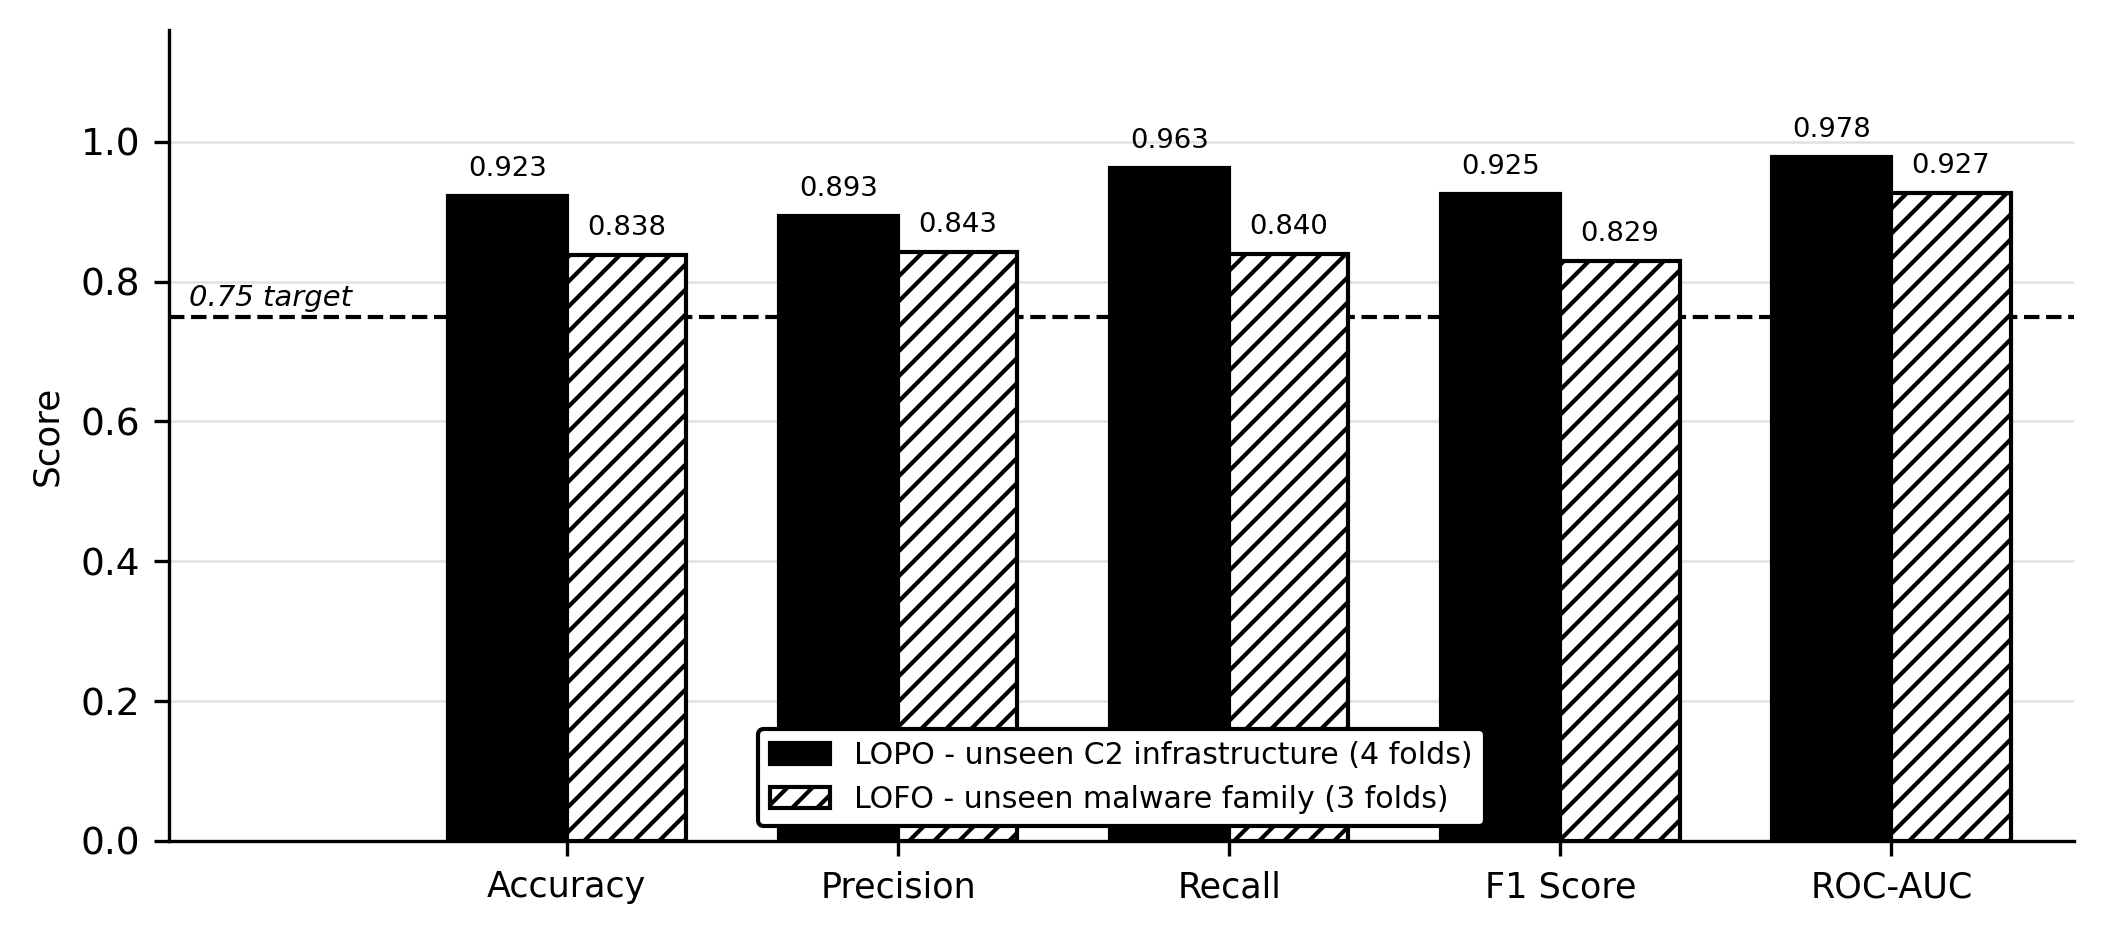
\includegraphics[width=\columnwidth]{figures/fig2_headline_results.png}
\caption{Class-balanced held-out performance of the deployed model. Both protocols apply the same reliability rule: a fold enters a mean only if it contains at least ten positive test windows.}
\label{fig:headline}
\end{figure}

\subsection{Protocol}
Test sets are class-balanced -- benign windows are subsampled to the positive count, and five independent draws are averaged -- so that accuracy and precision are meaningful numbers rather than a restatement of a sub-1\% prevalence. Decision thresholds are always chosen by inner grouped cross-validation on training data only, and never on the fold being scored. Two held-out protocols are reported: \textbf{LOPO} (leave-one-C2-source-out), which holds out one communicating pair at a time and represents the common operational case of a known family reaching new infrastructure; and \textbf{LOFO} (leave-one-malware-family-out), which holds out an entire family and represents the harder case of a family never seen in training.

One reliability rule is applied uniformly to both protocols: a fold contributes to a reported mean only if it contains at least ten positive test windows, because a fold containing three positives cannot distinguish a working detector from a fortunate one. Of the 50 in-scope C2 pairs, 15 contain enough positives to form a LOPO fold at all, and four of those clear the ten-positive bar; of the six malware families, three clear it. All means in Table \ref{tab:headline} are taken over those folds only.

\subsection{Headline results}
Table \ref{tab:headline} and Fig.~\ref{fig:headline} report both protocols for the deployed model. Every reported mean exceeds the 0.75 target set for this component on every metric, but two qualifications are important.

First, applying the reliability rule to LOPO is not a cosmetic choice. Averaging all 15 pair folds instead -- including the 11 that contain only three positive windows each, and on which the model is trivially correct -- would report 96.2\% accuracy and 0.991 ROC-AUC, visibly higher on every metric. That figure is listed in Table \ref{tab:headline} for transparency, but we regard it as inflated by folds too small to carry information and do not claim it.

Second, the mean is not the whole story. One held-out family, ZeusV1, reaches only 60.2\% recall and 71.1\% F1, below the target, even though it does not pull the three-family mean below it. ZeusV1 is also the largest held-out family, contributing 226 of the 330 in-scope positive windows across three distinct C2 servers, so it is the best-supported single measurement in the LOFO set rather than a small-sample outlier. We report it rather than averaging it away.

\begin{table}[t]
\caption{Deployed model, class-balanced held-out evaluation. LOPO holds out one C2 source; LOFO holds out an entire malware family. Means cover only folds with at least ten positive test windows; the final row is shown for transparency and is not claimed.}
\label{tab:headline}
\centering
\footnotesize
\setlength{\tabcolsep}{3.4pt}
\begin{tabular}{lccccc}
\toprule
\textbf{Protocol} & \textbf{Acc.} & \textbf{Prec.} & \textbf{Rec.} & \textbf{F1} & \textbf{AUC} \\
\midrule
LOPO (4 folds) & 92.3\% & 89.3\% & 96.2\% & 92.5\% & 0.978 \\
LOFO (3 folds) & 83.8\% & 84.3\% & 84.0\% & 82.9\% & 0.927 \\
\midrule
\quad ZeusV1 fold only & 75.5\% & 86.9\% & 60.2\% & 71.1\% & 0.887 \\
\quad LOPO, all 15 folds & 96.2\% & 94.8\% & 99.0\% & 96.6\% & 0.991 \\
\bottomrule
\end{tabular}
\end{table}

\subsection{Why XGBoost: a five-classifier comparison}
Logistic regression, Naive Bayes, a decision tree, Random Forest, and XGBoost were trained on the identical scoped corpus, with identical features and identical sample weights, and with no per-model threshold tuning: a fixed 0.5 threshold at natural prevalence. This is a different, uncalibrated protocol from Table \ref{tab:headline} and is included only to justify the architecture choice. Table \ref{tab:classifiers} and Fig.~\ref{fig:classifiers} report the result. Random Forest wins the optimistic grouped split (F1 0.688, AUC 0.996) and then predicts \emph{zero} positives on every held-out family: precision, recall, and F1 are all exactly 0.000 across all six families, despite a still-informative ROC-AUC of 0.740. Its ranking survives the family shift, but no unseen-family window ever crosses 0.5. The split AUC of Naive Bayes (0.467, worse than chance) reflects its independence assumption being violated by strongly correlated timing features. XGBoost has both the best LOFO ROC-AUC (0.858) and the best LOFO F1 (0.267) of the five under this protocol, and that is the basis for its selection: cross-family ranking rather than in-distribution accuracy.

\begin{figure}[t]
\centering
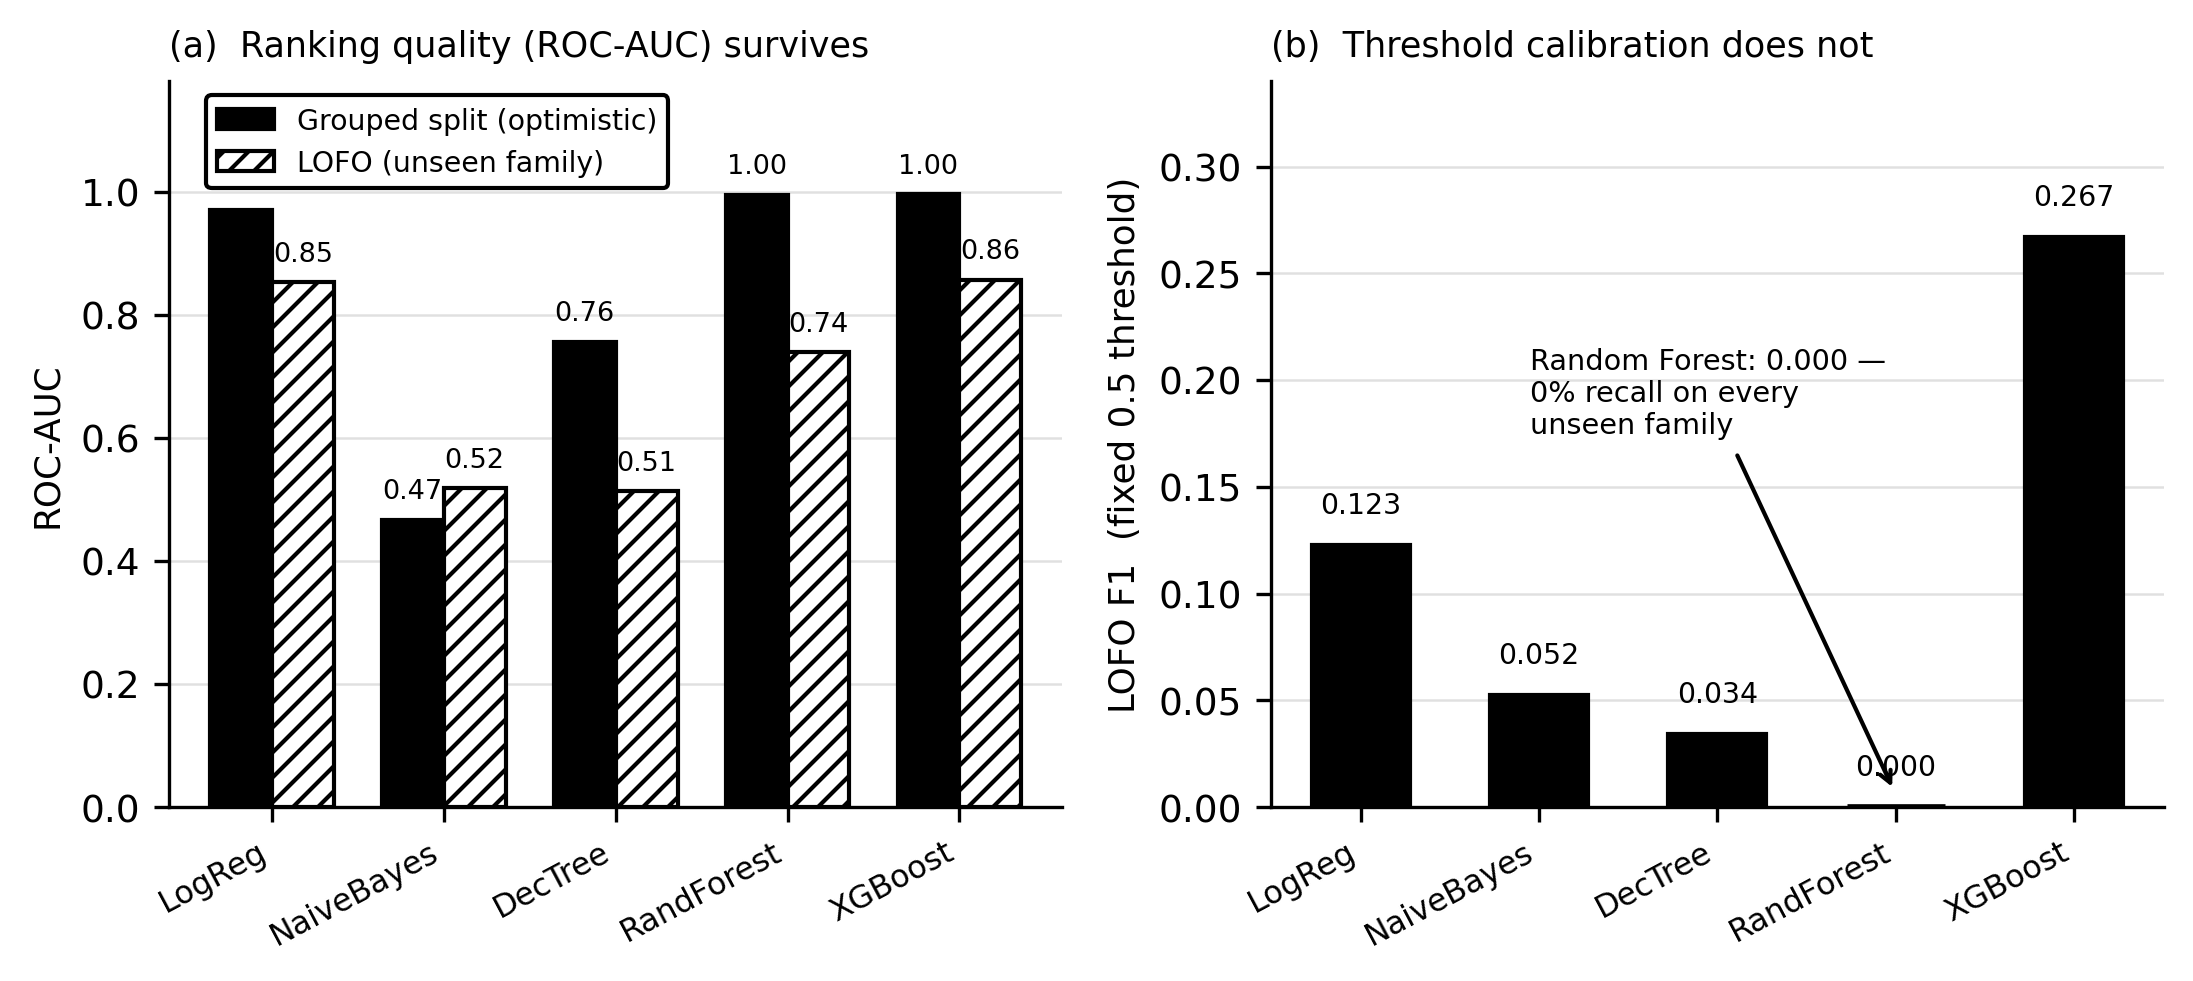
\includegraphics[width=\columnwidth]{figures/fig3_classifier_comparison.png}
\caption{Five classifiers on the identical scoped dataset and weighting. Random Forest wins the optimistic split, then fails to generalise: ranking quality partly survives an unseen family, but calibration to a fixed threshold does not.}
\label{fig:classifiers}
\end{figure}

\begin{table}[t]
\caption{Five classifiers, identical scoped data, fixed 0.5 threshold}
\label{tab:classifiers}
\centering
\small
\begin{tabular}{lccc}
\toprule
\textbf{Classifier} & \textbf{Split F1} & \textbf{LOFO F1} & \textbf{LOFO AUC} \\
\midrule
Logistic Regression & 0.096 & 0.123 & 0.853 \\
Naive Bayes & 0.024 & 0.052 & 0.518 \\
Decision Tree & 0.640 & 0.034 & 0.514 \\
Random Forest & \textbf{0.688} & 0.000 & 0.740 \\
XGBoost (deployed) & 0.452 & \textbf{0.267} & \textbf{0.858} \\
\bottomrule
\end{tabular}
\end{table}

\subsection{Fusion weight and a structural limit}
The ML weight was swept from 0.45 to 0.70 through the real fusion function on the full scoped corpus, under an assumed idle-background browser context. BEACON F1 peaks at a weight of 0.55 (0.9745, against 0.9324 at the previous value of 0.45); beyond 0.55, precision falls faster than recall rises. This is the weight deployed in Section III-C.

Separately, under a context-blind condition in which no browser-context fields are available -- the most that any network-only capture could ever supply -- confirmed-BEACON recall measures \textbf{exactly 0.000 at every tested weight from 0.45 to 0.70}. This is not a training artefact: it follows from the both-signal corroboration guard withholding confirmation whenever the heuristic term sits at its floor, independently of how the two weights are divided. SUSPICIOUS-tier detection is unaffected across the same range (F1 between 0.947 and 0.967), so nothing is silently missed; it surfaces at a lower confidence tier instead. We take this as the central operational claim of the paper: no re-weighting of the fusion substitutes for the browser-execution context that the architecture is built to supply.

\section{Limitations}

\begin{itemize}
\item One held-out family, ZeusV1, falls below the 0.75 target on recall and F1, although the aggregate mean clears it (Section VI-B). Because it is the largest held-out family, this is a real limit of cross-family generalisation rather than a sampling artefact.
\item Three of the six families are too small to evaluate meaningfully and are excluded from all reported means: Sogou and ZeusB26, with three held-out positive windows each, and Zeus78, which retains one window after the scope criterion is applied.
\item Detection scope is active, periodic C2. A channel that never completes an exchange lies outside the trained concept, although it is separately shown to remain detectable (Section IV-C).
\item Confirmed BEACON detection architecturally requires corroborating browser context and is unreachable from the model alone without it (Section VI-D), which is a limitation for any deployment that cannot instrument the browser.
\item The corpus predates modern jittered and malleable C2 frameworks. Extending coverage requires new labelled captures rather than further mining of the present ones.
\end{itemize}

\section{Conclusion}

Evaluating a browser-execution-aware C2 detector by unseen malware family and unseen infrastructure, rather than by a random split, did more than lower a number: it surfaced a pseudo-replicated training corpus, an out-of-scope traffic concept hiding inside the positive class, and a calibration-specific threshold bug, each diagnosed from first principles and corrected. Applying one reliability rule uniformly to both held-out protocols, the corrected and calibrated model reaches 92.3\% accuracy on unseen infrastructure and 83.8\% on an unseen malware family, class-balanced and leakage-free; we also report, and decline to claim, the higher figure that a less careful aggregation would have produced. A five-architecture comparison shows that the deployed classifier was chosen for surviving family shift rather than for winning an optimistic split, since the alternative that wins the split generalises to nothing. We close with a structural rather than incidental limitation, measured directly: no fusion weight recovers confirmed detection from the model alone once browser context is unavailable, which restates the argument of this paper as an engineering fact.

\section*{Acknowledgment}
The authors thank the members of research group R26-CS-003 for their collaboration on the shared WebSentinel platform, and the Stratosphere Laboratory for the public captures on which this work depends.

\bibliographystyle{IEEEtran}
\bibliography{references}

\end{document}
